
\chapter{Discrete process measurement}

\label{Process_switches}

The word ``discrete'' means \textit{individual} or \textit{distinct}.  In engineering, a ``discrete'' variable or measurement refers to a true-or-false condition.  Thus, a discrete sensor is one that is only able to indicate whether the measured variable is above or below a specified setpoint. \index{Discrete}

Discrete sensors typically take the form of \textit{switches}, built to ``trip'' when the measured quantity either exceeds or falls below a specified value.  These devices are less sophisticated than so-called \textit{continuous} sensors capable of reporting an analog value, but they are quite useful in industry. \index{Switch}

Many different types of discrete sensors exist, detecting variables such as position, fluid pressure, material level, temperature, and fluid flow rate.  The output of a discrete sensor is typically electrical in nature, whether it be an active voltage signal or just resistive continuity between two terminals on the device.








\filbreak
\section{``Normal'' status of a switch}

\label{normal_switch}

Perhaps the most confusing aspect of discrete sensors is the definition of a sensor's \textit{normal} status.  Electrical switch contacts are typically classified as either \textit{normally-open} or \textit{normally-closed}, referring to the open or closed status of the contacts under ``normal'' conditions.  But what exactly defines ``normal'' for a switch?  The answer is not complex, but is often misunderstood due to the ambiguous nature of the word \textit{normal}.  \index{Normal state of a switch}

The ``normal'' status for a switch is the status its electrical contacts are in \textit{during a condition of no physical stimulation}.  Another way to think of the ``normal'' status is to think in terms of the switch being \textit{at rest}.  For a momentary-contact pushbutton switch, this would be the status of the switch contact when it is \textit{not} being pressed.  Electrical switches are always drawn in schematic diagrams in their ``normal'' statuses, regardless of their application.  For instance, the following diagram shows a normally-open pushbutton switch controlling a lamp on a 120 volt AC circuit (the ``hot'' and ``neutral'' poles of the AC power source labeled L1 and L2, respectively):

$$
\includegraphics{discrete01.eps}$$

We can tell this switch is a normally-open (NO) switch because it is drawn in an open position.  The lamp will energize only if someone presses the switch, holding its normally-open contacts in the ``closed'' position.  Normally-open switch contacts are sometimes referred to in the electrical industry as \textit{form-A} contacts. \index{Form-A switch contact}

If we had used a normally-closed pushbutton switch instead, the behavior would be exactly opposite.  The lamp would energize if the switch was left alone, but it would turn off if anyone pressed the switch.  Normally-closed switch contacts are sometimes referred to in the electrical industry as \textit{form-B} contacts:  \index{Form-B switch contact}

$$
\includegraphics{discrete02.eps}$$

This seems rather simple, don't you think?  What could possibly be confusing about the ``normal'' status of a switch?  The confusion becomes evident, though, when you begin to consider \textit{process} switches (i.e. switches actuated by process measurements such as pressure, flow, level, etc.).  In order to better understand this concept, we will consider a simple application of a \textit{flow} switch: a switch built to actuate when a sufficient rate of fluid flows through a pipe.  \index{Process switch} \index{Switch, process}

\filbreak

A flow switch is built to detect fluid flow through a pipe.  In a schematic diagram, the switch symbol appears to be a toggle switch with a ``flag'' hanging below.  The schematic diagram, of course, only shows the circuitry and not the pipe where the switch is physically mounted:

$$\includegraphics{discrete03.eps}$$

This particular flow switch is used to trigger an alarm light if coolant flow through the pipe ever falls to a dangerously low level, and the contacts are \textit{normally-closed} as evidenced by the closed status in the diagram.  Here is where things get confusing: even though this switch is designated as ``normally-closed,'' it will spend most of its lifetime being held in the open status by the presence of adequate coolant flow through the pipe.  Only when the flow through the pipe slows down enough will this switch return to its ``normal'' status and conduct electrical power to the lamp.  In other words, the ``normal'' status for this switch (closed) is actually an \textit{abnormal} status for the process it operates within (low flow), for the simple reason that the switch should be stimulated and not at rest while the process is operating as it should.  

Students often wonder why process switch contacts are labeled according to this convention of ``no stimulation'' instead of according to the typical status of the process in which the switch is used.  The answer to this question is that the manufacturer of the switch has no idea whatsoever as to your intended use.  A flow switch manufacturer does not know or care whether their product gets used as a low-flow detector or as a high-flow detector.  In other words, the manufacturer cannot predict what the typical status of \textit{your} process will be, and so the definition of ``normal'' status for the switch must be founded on some common criterion unrelated to your particular application.  That common criterion is the resting status: when the sensor is exposed to the \textit{least} (or no) amount of stimulation from the process it senses.

\vskip 10pt

Here is a listing of ``normal'' definitions for various process switch types:

\begin{itemize}
\item \textbf{Limit switch}: target not contacting the switch
\item \textbf{Proximity switch}: target far away
\item \textbf{Pressure switch}: low pressure (or even a vacuum)
\item \textbf{Level switch}: low level (empty)
\item \textbf{Temperature switch}: low temperature (cold)
\item \textbf{Flow switch}: low flow rate (fluid stopped)
\end{itemize}

These are the conditions represented by the switch statuses shown in a schematic diagram.  These may very well \textit{not} be the statuses of the switches when they are exposed to \textit{typical} operating conditions in the process.

\filbreak

A helpful tip to remember about process switches and their respective schematic diagram symbols is that the symbols are conventionally drawn in such a way that an \textit{upward} motion of the movable switch element represents \textit{increasing stimulus}.  Here are some examples of this, showing various process switch types and NO/NC contact configurations, comparing their states with no stimulus versus when the stimulus exceeds the each switch's threshold or ``trip'' setting.  The \textit{normal} status of each switch as defined by the manufacturer is labeled in green text:

$$\includegraphics{discrete32.eps}$$

It is imperative\footnote{Mistaken interpretations of switch status remains one of the most resilient misconceptions for students first learning this topic.  It seems that a great many students prefer to think of a switch's drawn status as its status at the present moment (e.g. when the process is running as expected).  I believe the heart of this misconception is the meaning of the word ``normal,'' which to most peoples' minds refers to ``the way things typically are.''} to remember that the way a switch is drawn in a schematic diagram merely represents its ``normal'' status as defined by the manufacturer.  This may or may not be the switch's status during ``typical'' operation of the process, and it may or may not be the status of that switch at the time of concern when you are examining the schematic!  The ``normal'' status of a switch means just one thing: what that switch will do when subjected to minimum stimulus -- that is to say, what it will do when its stimulus is less than the actuation threshold of the switch.  \index{Normal state of a switch}

\filbreak

For example, the LED in this circuit will turn on if the liquid level rises above 14 inches \textit{and} the pressure falls below 22 PSI \textit{and} either the flow is less than 3 gallons per minute \textit{or} the temperature is greater than 125 degrees Fahrenheit:

$$\includegraphics{discrete33.eps}$$

Since we know we need a switch to be \textit{closed} in order to conduct electricity and provide a path for current in this circuit, we are looking for the necessary conditions to close each switch.  For any normally-closed (NC) switch, this means a stimulus value less than the actuation threshold.  For any normally-open (NO) switch, this means a stimulus value great enough to exceed the threshold and ``hold'' the switch in its actuated state.  Since the flow and pressure switches in this circuit are both NC, we are looking for flow and pressure values less than the respective settings.  Since the level and temperature switches are both NO, we are looking for level and temperature values in excess of their respective settings.

\vskip 10pt

The present status of a switch may be determined by comparing its stimulating quantity against its trip (threshold) setting.  A switch will be in its ``normal'' (resting) state when the stimulus value is less than the threshold value.  Conversely, a switch will be in its ``actuated'' state when the stimulus value exceeds the threshold value.  Determination of a switch's status, therefore, is a matter of comparing the stimulus quantity to the threshold ``trip'' setting.  One cannot simply look at the schematic diagram to tell what the switch is doing -- one must \textit{compare} the switch's setting versus against a known stimulus value in order to tell whether it will be in its resting state or not.

Likewise, if we happen to know the switch's present status in a system, we may qualitatively determine the stimulating quantity by comparing the present status against the ``normal'' (resting) status.  If a switch is in its resting state, then the stimulating quantity must be less than the trip threshold.  If a switch is in its actuated (non-normal) state, then the stimulating quantity must be greater than the trip threshold\footnote{In this discussion I am deliberately omitting the detail of \textit{deadband} for process switches, for the sake of simplicity.}.  The next example showcases these determinations.

\filbreak

In this next example, we see a pictorial representation of multiple switches wired to the discrete input channels of a programmable logic controller (PLC), with red LED indicators denoting the real-time status of each input on the PLC:

$$\includegraphics{discrete34.eps}$$

We may determine a switch's degree of stimulation by comparing its present status with its ``normal'' status.  If a switch happens to be in the same state as its normal state (i.e. resting), we know its stimulus must be less than the threshold (trip) value.  If a switch happens to be in the opposite state as its normal state (i.e. actuated), we know its stimulus has exceeded the threshold (trip) value.  The states of these four switches may be shown in a table:

% No blank lines allowed between lines of an \halign structure!
% I use comments (%) instead, so that TeX doesn't choke.

$$\vbox{\offinterlineskip
\halign{\strut
\vrule \quad\hfil # \ \hfil & 
\vrule \quad\hfil # \ \hfil & 
\vrule \quad\hfil # \ \hfil & 
\vrule \quad\hfil # \ \hfil & 
\vrule \quad\hfil # \ \hfil \vrule \cr
\noalign{\hrule}
%
% First row
\textbf{Switch} & \textbf{Normal status} & \textbf{Present status} & \textbf{Trip value} & \textbf{Stimulus} \cr
%
\noalign{\hrule}
%
% Another row
Pressure & Normally-closed (NC) & Closed & 12 PSI & $P <$ 12 PSI \cr
%
\noalign{\hrule}
%
% Another row
Temperature & Normally-open (NO) & Closed & 235 $^{o}$F & $T >$ 235 $^{o}$F \cr
%
\noalign{\hrule}
%
% Another row
Level & Normally-closed (NC) & Closed & 4 inches & $L <$ 4 inches \cr
%
\noalign{\hrule}
%
% Another row
Limit & Normally-open (NO) & Open & n/a & \textit{no contact} \cr
%
\noalign{\hrule}
} % End of \halign 
}$$ % End of \vbox




\filbreak
\section{Hand switches}

A \textit{hand switch} is exactly what the name implies: an electrical switch actuated by a person's hand motion.  These may take the form of toggle, pushbutton, rotary, pull-chain, etc.  A common form of industrial pushbutton switch looks something like this: \index{Hand switch}

$$\includegraphics{discrete04.eps}$$

The threaded neck inserts through a hole cut into a metal or plastic panel, with a matching nut to hold it in place.  Thus, the button faces the human operator(s) while the switch contacts reside on the other side of the panel.

When pressed, the downward motion of the actuator breaks the electrical bridge between the two NC contacts, forming a new bridge between the NO contacts:

$$\includegraphics{discrete05.eps}$$

The schematic diagram symbol for this type of switch looks much like the real thing, with the normally-closed contact set on top and the normally-open contact set below:  \index{Normal state of a switch}

$$
\includegraphics{discrete06.eps}$$

\filbreak

Connecting two of the terminals together makes this form of switch electrically identical to a \textit{Form C}:

$$\includegraphics{discrete28.eps}$$

This switch contact arrangement is sometimes referred to as a \textit{form-C} contact set, since it incorporates both a form-A contact (normally-open) as well as a form-B contact (normally-closed). \index{Form-C switch contact}

\filbreak

Most industrial hand switches are available in modular form, where sets of switch contact blocks may be ``stacked'' together to be actuated by the same pushbutton or rotary knob.  This allows an almost unlimited number of switch contacts to be simultaneously actuated by a single actuating mechanism.  Different actuator types such as pushbuttons, rotary selectors, knobs, and keyswitches may also be interchanged with contact modules for maximum flexibility:

$$\includegraphics{discrete27.eps}$$






\filbreak
\section{Limit switches}

$$\includegraphics{discrete10.eps}$$

A \textit{limit switch} detects the physical motion of an object by direct contact with that object.  An example of a limit switch is the switch detecting the open position of an automobile door, automatically energizing the cabin light when the door opens.  \index{Limit switch}

Recall from section \ref{normal_switch} that the ``normal'' status of a switch is the resting condition of \textit{no stimulation}.  A limit switch will be in its ``normal'' status when it is not in contact with anything (i.e. nothing touching the switch actuator mechanism).  \index{Normal state of a switch}

Limit switches find many uses in industry, particular in robotic control and CNC (Computer Numerical Control) machine tool systems.  In many motion-control systems, the moving elements have ``home'' positions where the computer assigns a position value of zero.  For example, the axis controls on a CNC machine tool such as a lathe or mill all return to their ``home'' positions upon start-up, so the computer can know with confidence the starting locations of each piece.  These home positions are detected by means of limit switches.  The computer commands each servo motor to travel fully in one direction until a limit switch on each axis trips.  The position counter for each axis resets to zero as soon as the respective limit switch detects that the home position has been reached.  \index{Home position, CNC machine}

A typical limit switch design uses a roller-tipped lever to make contact with the moving part.  Screw terminals on the switch body provide connection points with the NC and NO contacts inside the switch.  Most limit switches of this design share a ``common'' terminal between the NC and NO contacts like this:

$$\includegraphics{discrete07.eps}$$

This switch contact arrangement is sometimes referred to as a \textit{form-C} contact set, since it incorporates both a form-A contact (normally-open) as well as a form-B contact (normally-closed). \index{Form-C switch contact}

\filbreak

A close-up view of several limit switches (used on a drum sequencer) shows the arrangement of connection terminals for form-C contacts.  Each limit switch has its own ``NO'' (normally-open), ``NC'' (normally-closed), and ``C'' (common) screw terminal for wires to attach:

$$\includegraphics[width=4in]{form_c_contacts.eps}$$

A limit switch assembly attached to the stem of a rotary valve -- used to detect the fully-closed and fully-open positions of the valve -- is shown in the following photograph:

$$\includegraphics[width=4in]{limit_switch_1.eps}$$








\filbreak
\section{Proximity switches}

A \textit{proximity switch} is one detecting the proximity (closeness) of some object.  By definition, these switches are \textit{non-contact sensors}, using magnetic, electric, or optical means to sense the proximity of objects. \index{Proximity switch}

Recall from section \ref{normal_switch} that the ``normal'' status of a switch is the resting condition of \textit{no stimulation}.  A proximity switch will be in its ``normal'' status when it is distant from any detectable object.  \index{Normal state of a switch}

Being non-contact in nature, proximity switches are often used instead of direct-contact limit switches for the same purpose of detecting the position of a machine part, with the advantage of never wearing out over time due to repeated physical contact.  

Most proximity switches are \textit{active} in design.  That is, they incorporate a powered electronic circuit to sense the proximity of an object.  \textit{Inductive} proximity switches sense the presence of metallic objects through the use of a high-frequency magnetic field.  \textit{Capacitive} proximity switches sense the presence of non-metallic objects through the use of a high-frequency electric field.  \textit{Optical} proximity switches detect the interruption of a light beam by an object.  \textit{Ultrasonic} proximity switches sense the presence of dense matter by the reflection of sound waves.

The schematic diagram symbol for a proximity switch with mechanical contacts is the same as for a mechanical limit switch, except the switch symbol is enclosed by a diamond shape, indicating a powered (active) device:

$$\includegraphics{discrete08.eps}$$

Many proximity switches, though, do not provide ``dry contact\footnote{This curious label is used to describe switch contacts lacking their own built-in power source, as opposed to a switch contained in a device that also provides power to drive the switch circuit.  Dry contacts may be mechanical in nature, or they may be electronic (e.g. transistor).  By contrast, a ``wet'' contact is one already connected to an internal power source, ready to drive a load with no other external components needed.}'' outputs.  Instead, their output elements are transistors configured either to \textit{source} current or \textit{sink} current.  The terms ``sourcing'' and ``sinking'' are best understood by visualizing electric current in the direction of \textit{conventional flow} rather than \textit{electron flow}.  \index{Dry contact}  \index{Switch, dry contact}  \index{Wet contact}  \index{Switch, wet contact}

\filbreak

The following schematic diagrams contrast the two modes of switch operation, using red arrows to show the direction of current (conventional flow notation).  In both examples, the load being driven by each proximity switch is a light-emitting diode (LED): \index{Conventional flow} \index{Electron flow} \index{Sourcing output switch} \index{Sinking output switch}

$$\includegraphics{discrete09.eps}$$

A common coloring convention for electronic proximity switches is brown for +V power supply, blue for ground ($-$ pole of power supply), and black for the switched output signal.  This convention is common to sinking and sourcing proximity switches alike.

An electronic switch designed to sink current through its signal wire is alternatively referred to as an \textit{NPN} switch due to the type of transistor used in its output.  Conversely, an electronic switch designed to source current through its signal wire may be referred to as a \textit{PNP} switch.  The key to understanding these labels is to recognize the emitter terminal of the output transistor is always the one connected to the power supply rail.  For a sinking switch, this means the emitter must connect to the negative rail, necessitating\footnote{To be honest, one \textit{could} use an NPN transistor to source current or a PNP to sink, but it would require the transistor be used in the \textit{common-collector} configuration which does not allow for saturation.  The engineers designing these proximity switches strive for complete saturation of the transistor, in order to achieve minimum ``on'' resistance, and that requires a common-emitter configuration.} an NPN transistor to do the switching.  For a sourcing switch, this means the emitter must connect to the positive rail, in which case only a PNP transistor will suffice.  \index{PNP output switch}  \index{NPN output switch}

\filbreak

Yet another convention for describing sourcing and sinking transistor switches is to refer to them as \textit{high-side} switches and \textit{low-side} switches, respectively.  A sourcing transistor (PNP) has its emitter terminal attached directly to the ``high'' rail (+) of the DC power supply.  A sinking transistor (NPN), by contrast, has its emitter terminal attached directly to the ``low'' rail ($-$) of the DC power supply.  \index{High-side transistor switch}  \index{Low-side transistor switch}

$$\includegraphics{discrete29.eps}$$

\filbreak

These photographs show two different styles of electronic proximity switch:

$$\includegraphics[width=2.5in]{prox_switch_3.eps} \hskip 30pt \includegraphics[width=2.5in]{prox_switch_1.eps}$$

Many industrial proximity switches have built-in LED indicator lamps to help technicians diagnose circuit problems by directly indicating switch status.  With just a glance, one may tell whether or not the proximity switch is detecting the presence of an object.

\filbreak

The next photograph shows a proximity switch detecting the passing of teeth on a chain sprocket, generating a slow square-wave electrical signal as the sprocket rotates.  Such a switch may be used as a rotational speed sensor (sprocket speed proportional to signal frequency) or as a broken chain sensor (when sensing the rotation of the driven sprocket instead of the drive sprocket):

$$\includegraphics[width=5in]{prox_switch_2.eps}$$

\vskip 10pt

Like other types of process switches, proximity switches come in both ``normally open'' (NO) and ``normally closed'' (NC) varieties.  This distinction has nothing whatsoever to do with sourcing versus sinking (PNP vs. NPN), but rather what the status of the proximity switch will be when no objects are near.  Thus, it is possible to find normally-open proximity switches that are sinking (NPN) as well as normally-open proximity switches that are sourcing (PNP), and normally-closed proximity switches in either sinking or sourcing designs as well.

These switch characteristics are commonly fixed, and must be specified when ordering the device.  Likewise, the detection range of a proximity switch is usually a fixed parameter rather than being adjustable.

%\vskip 10pt

% ADD: NAMUR proximity sensors
%   --> Actually analog sensors with variable DC current output
%   --> require connection to an amplifier unit to convert to discrete (on/off) output
%   --> Very low current means low risk of creating an explosion-inducing spark







\filbreak
\section{Pressure switches}

A \textit{pressure switch} is one detecting the presence of fluid pressure.  Pressure switches often use diaphragms or bellows as the pressure-sensing element, the motion of which actuates one or more switch contacts. \index{Pressure switch}

Recall from section \ref{normal_switch} that the ``normal'' status of a switch is the resting condition of \textit{no stimulation}.  A pressure switch will be in its ``normal'' status when it senses minimum pressure (e.g. an applied pressure, or in some cases a vacuum condition)\footnote{If the trip setting of a pressure switch is below atmospheric pressure, then it will be ``actuated'' at atmospheric pressure and in its ``normal'' status only when the pressure falls below that trip point (i.e. a vacuum).}.  For a pressure switch, ``normal'' status is any fluid pressure \textit{below} the trip threshold of the switch.  \index{Normal state of a switch}

$$\includegraphics{discrete11.eps}$$

The following photograph shows two pressure switches sensing the same fluid pressure as an electronic pressure transmitter (the device on the far left) because they are all plumbed to a common tube:

$$\includegraphics[width=5in]{press_switch_1.eps}$$

\filbreak

A legacy design of pressure switch uses a bourdon tube as the pressure-sensing element, and a glass bulb partially filled with mercury as the electrical switching element.  When applied pressure causes the bourdon tube to flex sufficiently, the glass bulb tilts far enough to cause the mercury to fall against a pair of electrodes, thus completing an electrical circuit.  A great many pressure switches of this design were sold under the brand name of ``Mercoid,'' with a few appearing in this photograph of a steam boiler (the round-shaped units with glass covers allowing inspection of the bourdon tube and mercury tilt switch):  \index{Mercury tilt switch}  \index{Tilt switch, mercury}  \index{Mercoid pressure switch}

$$\includegraphics[width=5in]{pressure_switch_4.eps}$$

\filbreak

A close-up photograph of one of these pressure switches appears here.  The bourdon tube is grey in color, and almost as wide in diameter as the circular switch housing.  The mercury tilt switch bottles have yellow-colored plastic caps covering up their external electrical contacts:

$$\includegraphics[width=5in]{pressure_switch_5.eps}$$

The next set of photographs show a mercury tilt switch removed from the pressure switch mechanism, so you may see the switch in two different states (contact open on the left, and closed on the right):

$$\includegraphics[width=2.5in]{tilt_switch_1.eps} \hskip 30pt 
\includegraphics[width=2.5in]{tilt_switch_2.eps}$$

Advantages of mercury tilt switches include immunity to switch contact degradation from harmful atmospheres (oil mist, dirt, dust, corrosion) as well as safety in explosive atmospheres (since a spark contained within a hermetically sealed glass bulb cannot touch off an explosion in the surrounding atmosphere).  Disadvantages include the possibility of intermittent electrical contact resulting from mechanical vibration, as well as sensitivity to mounting angle (i.e. you would \textit{not} want to use this kind of switch aboard a moving vehicle!).

\filbreak

A pressure switch manufactured by the Danfoss corporation appears in the next photograph.  This particular model of pressure switch has windows on the front cover allowing a technician to see the pressure limit setting inside:  \index{Danfoss pressure switch}

$$\includegraphics[width=3in]{pressure_switch_3.eps}$$

This switch balances the force generated by a pressure-sensing element against a mechanical spring.  Tension on the spring may be adjusted by a technician, which means the trip point of this switch is adjustable.

One of the settings on this switch is the \textit{deadband} or \textit{differential} pressure setting, seen in the lower window.  This setting determines the amount of pressure change required to re-set the switch to its normal state after it has tripped.  For example, a high-pressure switch with a trip point of 67 PSI (changes state at 67 PSI, increasing) that re-sets back to its normal state at a pressure of 63 PSI decreasing has a ``deadband'' or ``differential'' pressure setting of 4 PSI (67 PSI $-$ 63 PSI = 4 PSI).  \index{Deadband setting, pressure switch}  \index{Differential setting, pressure switch}

\filbreak

The ``differential'' pressure setting of a gauge pressure switch is not to be confused with a true \textit{differential pressure} switch.  In the next photograph, we see a pressure switch truly actuated by \textit{differential} pressure (the difference in fluid pressure sensed between two ports):  \index{Differential pressure switch}

$$\includegraphics[width=3in]{pressure_switch_2.eps}$$

The electrical switch element is located underneath the blue cover, while the diaphragm pressure element is located within the grey metal housing.  The net force exerted on the diaphragm by the two fluid pressures varies in magnitude and direction with the magnitude of those pressures.  If the two fluid pressures are precisely equal, the diaphragm experiences no net force (zero differential pressure).

Like the Danfoss gauge pressure switch seen previously, this differential pressure switch has a ``trip'' or ``limit'' setting as well as a ``dead-band'' or ``differential'' setting.  It is important to recognize and clearly distinguish the two meanings of \textit{differential pressure} in the context of this device.  It senses differences in pressure between two input ports (``differential pressure'' -- the difference between two different fluid pressure connections), but being a switch, it also exhibits some dead band in its action (``differential pressure'' -- a change in pressure required to re-set the switch's state).







\filbreak
\section{Level switches}

\label{level_switch}

A \textit{level switch} is one detecting the level of liquid or solid (granules or powder) in a vessel.  Level switches often use floats as the level-sensing element, the motion of which actuates one or more switch contacts. \index{Level switch}

Recall from section \ref{normal_switch} that the ``normal'' status of a switch is the resting condition of \textit{no stimulation}.  A level switch will be in its ``normal'' status when it senses minimum level (e.g. an empty vessel).  For a level switch, ``normal'' status is any fluid level \textit{below} the trip threshold of the switch.  \index{Normal state of a switch}

$$\includegraphics{discrete12.eps}$$






\filbreak
\subsection{Float-type level switches}

Some level switches use a \textit{float} to sense the level of a liquid surface, actuating an electrical switch by the motion of the float.  The electrical schematic symbol for a level switch is actually based on this type of mechanism, with a round ``ball'' float drawn as the actuating element:

$$\includegraphics{discrete12.eps}$$

An example of this technology is a level switch manufactured by Magnetrol, with two such switches shown in the following photograph of a steam boiler.  These switches sense water level in the steam drum of the boiler: \index{Magnetrol liquid level switch}

$$\includegraphics[width=5in]{level_switch_1.eps}$$

\filbreak

The Magnetrol float switch mechanism uses a mercury tilt bulb, tilted by a magnet's attraction to a steel rod lifted into position by a float.  The float directly senses liquid level, positioning the steel rod either closer to or farther away from the magnet.  If the rod comes close enough to the magnet, the mercury bottle tilts to change the switch's electrical status:  \index{Mercury tilt switch}  \index{Tilt switch, mercury}

$$\includegraphics{level_switch_8.eps}$$

A feature of this design is complete isolation between the electrical components and the ``wet'' components sensing the liquid level.  The steel rod moves inside a non-magnetic metal tube, with the tube sealing process fluid pressure from escape while still allowing the magnetic tilt switch to sense float position.

\vskip 10pt

Simpler float switch designs also exist for direct installation in open (vented) process vessels, resembling the float valve assembly on a water-flush toilet.  Any ``limit'' style switching element will work here, including inductive proximity switches, to sense the float's position in an environment where no isolation need exist between the switch and the process fluid(s):

$$\includegraphics{level_switch_9.eps}$$





\filbreak
\subsection{Tuning fork level switches}

This level switch uses a metal \textit{tuning fork} structure to detect the presence of a liquid or solid (powder or granules) in a vessel:  \index{Tuning fork level switch}  \index{Vibrating fork level switch}

$$\includegraphics[width=5in]{level_switch_2.eps}$$

An electronic circuit continuously excites the tuning fork, causing it to mechanically vibrate.  When the prongs of the fork contact anything with substantial mass, the resonant frequency of the fork decreases.  The circuit detects this frequency change and indicates the presence of mass contacting the fork.  The forks' vibrating motion tends to shake off any accumulated material, such that this style of level switch tends to be resistant to fouling.

\vskip 10pt

It should be noted that the previous photograph of the tuning-fork style level switch is complete: the fork ``paddles'' are only a couple of inches long and require no physical extensions in order to properly detect liquid or solid material at that point.







\filbreak
\subsection{Paddle-wheel level switches}

A more primitive variation on the theme of a ``tuning fork'' level switch is the \textit{rotating paddle} switch, used to detect the level of powder or granular solid material.  This level switch uses an electric motor to slowly rotate a metal paddle inside the process vessel.  If solid material rises to the level of the paddle, the material's bulk will place a mechanical load on the paddle.  A torque-sensitive switch mechanically linked to the motor actuates when enough torsional effort is detected on the part of the motor.  A great many level switches of this design sold in the United States under the trade-name \textit{Bindicator} (so-called because they detected the level of solid material in storage \textit{bins}).  \index{Rotating paddle level switch}

A ``Bindicator'' style of level switch appears in this photograph (painted black, against a white-painted hopper), used to detect the presence of soda ash powder in a hopper at a water treatment plant:

$$\includegraphics[width=5in]{level_switch_5.eps}$$






\filbreak
\subsection{Ultrasonic level switches}

Yet another style of electronic level switch uses ultrasonic sound waves to detect the presence of process material (either solid or liquid) at one point:  \index{Ultrasonic level switch}

$$\includegraphics[width=5in]{level_switch_3.eps}$$

Sound waves pass back and forth within the gap of the probe, sent and received by piezoelectric transducers.  The presence of any substance other than gas within that gap affects the received audio power, thus signaling to the electronic circuit within the bulkier portion of the device that process level has reached the detection point.  The lack of moving parts makes this probe quite reliable, although it may become ``fooled'' by heavy fouling.






\filbreak
\subsection{Capacitive level switches}

Another electronic liquid level switch technology is \textit{capacitive}: sensing level by changes in electrical capacitance between the switch and the liquid.  \index{Capacitive level switch}  The following photograph shows a couple of capacitive switches sensing the presence of water in a plastic storage vessel:

$$\includegraphics[width=4in]{level_switch_4.eps}$$







\filbreak
\subsection{Conductive level switches}

Perhaps the simplest (and oldest) form of electrical level detection is where a pair of metal electrodes contacts the process material to form a complete electrical circuit, actuating a relay.  This type of switch, of course, only works with granular solids and liquids that are electrically conductive (e.g. potable or dirty water, acids, caustics, food liquids, coal, metal powders) and not with non-conducting materials (e.g. ultra-pure water, oils, ceramic powders).

A legacy design for conductive level switches is the model 1500 ``induction relay'' originally manufactured by B/W Controls, using a special transformer/relay to generate an isolated AC probe voltage and sense the presence of liquid:  \index{B/W Controls model 1500 induction relay}  \index{Ametek model 1500 induction relay}

$$\includegraphics{level_switch_6.eps}$$

Line voltage (120 VAC) energizes the primary coil, sending a magnetic field through the laminated ferrous\footnote{``Ferrous'' simply means any iron-containing substance.} core of the relay.  This magnetic field easily passes through the center of the secondary coil when the secondary circuit is open (no liquid closing the probe circuit), thus completing the magnetic ``circuit'' in the core.  With the magnetic circuit thus completed, the armature will not be attracted to the core.  However, when a circuit is completed by liquid level rising to contact both probes, the secondary coil's resulting current ``bucks'' the magnetic flux\footnote{The reason for this opposition is rooted in the roles of primary and secondary coils as power \textit{load} and \textit{source}, respectively.  The voltage across each coil is a function of Faraday's Law of Electromagnetic Induction: $V = N{d \phi \over dt}$.  However, since the primary coil acts as a load (drawing power from the 120 VAC source) and the secondary coil acts as a source (sending power to the probes), the directions of current through the two coils will be opposite despite their common voltage polarities.  The secondary coil's opposite current direction causes an opposing magnetic force in that section of the core, reducing the magnetic flux there.  In a normal power transformer, this reduction in magnetic flux caused by secondary current is also felt by the primary coil (since there is only one magnetic ``path'' in a power transformer's core), which then causes the primary coil to draw more current and re-establish the core flux at its original magnitude.  With the inductive relay, however, the opposing magnetic force created by the secondary coil simply forces more of the primary coil's magnetic flux to bypass to the alternate route: through the armature.} through its center, causing more magnetic flux to bypass to the end poles where it attracts the ferrous armature toward the core frame.  This physical attraction actuates switch contacts which then signal the presence of liquid level at the probes.  \index{Faraday's Law of Electromagnetic Induction}

\filbreak

The following pair of illustrations shows the two conditions of this level switch, with the magnetic lines of flux highlighted as dashed lines through the core:

$$\includegraphics{level_switch_7.eps}$$

The ``transformer'' design of this particular conductive level switch not only provides electrical isolation between the probes and the energizing (120 VAC) circuit, but it also enables a wide range of detection voltages to be generated for the probes just by altering the number of wire ``turns'' in the secondary coil.  The B/W Controls model 1500 inductive relay is available in a variety of AC voltage output levels, ranging from 12 VAC (for detecting metallic substances) to 800 VAC for use with demineralized water such as that found in steam boiler systems.

\vskip 10pt

More modern variations on the same design theme use much lower AC voltages\footnote{The B/W Controls model 5200 solid-state relay, for example, uses only 8 volts AC at the probe tips.} to energize the probes, employing sensitive semiconductor amplifier circuits to detect probe current and signal liquid level.





%\filbreak
%\subsection{Optical (refractive) level switches}








\filbreak
\section{Temperature switches}

A \textit{temperature switch} is one detecting the temperature of some substance.  Temperature switches often use bimetallic strips as the temperature-sensing element, the motion of which actuates one or more switch contacts.  An alternative design uses a metal bulb filled with a fluid that expands with temperature, causing the switch mechanism to actuate based on the pressure this fluid exerts against a diaphragm or bellows.  This latter temperature switch design is really a pressure switch, whose pressure is a direct function of process temperature by virtue of the physics of the entrapped fluid inside the sensing bulb. \index{Temperature switch}

Recall from section \ref{normal_switch} that the ``normal'' status of a switch is the resting condition of \textit{no stimulation}.  A temperature switch will be in its ``normal'' status when it senses minimum temperature (i.e. cold, in some cases a condition colder than ambient)\footnote{If the trip setting of a temperature switch is below ambient temperature, then it will be ``actuated'' at ambient temperature and in its ``normal'' status only when the temperature falls below that trip point (i.e. colder than ambient).}.  For a temperature switch, ``normal'' status is any sensed temperature \textit{below} the trip threshold of the switch.  \index{Normal state of a switch}

$$\includegraphics{discrete13.eps}$$

\filbreak

The following photograph shows a temperature-actuated switch manufactured by the Ashcroft corporation:  \index{Ashcroft temperature switch}

$$\includegraphics[width=3in]{temp_switch_1.eps}$$

Like all other process switches, temperature switches exhibit a certain amount of \textit{deadband} in their switching action.  A temperature switch that trips at 300 $^{o}$F \textit{rising}, for example, will not re-set at 300 $^{o}$F \textit{falling}.  That switch would more likely reset at some lower temperature such as 295 $^{o}$F.  With mechanical switch designs, some amount of deadband is inevitable due to friction inside the mechanism.  However, process switch deadband is actually a useful characteristic as it helps avoid repeated ``nuisance'' alarms from happening.    \index{Deadband setting, temperature switch}

To understand this concept, it is helpful to imagine a scenario where the process variable is at or very near the trip point.  For our hypothetical temperature switch with a trip point of 300 $^{o}$F (rising), imagine a situation where the process temperature is precisely 300.0 $^{o}$F.  Any further rise in temperature will of course trip the switch (sounding an alarm).  With no deadband, however, the switch will immediately re-set when the temperature falls back down to 300.0 $^{o}$F.  This means the switch may possibly ``cycle'' back and forth between its trip and reset states with just a minute change in process temperature (300.0 $^{o}$F to 300.1 $^{o}$F and back again).  If the temperature switch is activating an alarm every time it trips, it will create a series of alarm events prompting operators to repeatedly acknowledge the alarm.  This is a nuisance to operations personnel, as it distracts them from addressing what they already realize is a process problem.  It is better for the switch to trip at 300.0 $^{o}$F rising \textit{and remain in that tripped state} until the temperature falls down to some degree substantially below the trip point.  This way, the operators only receive \textit{one} alarm event rather than multiple alarm events for each process temperature excursion.

Some mechanical temperature switches come equipped with a separate adjustment for deadband (also called \textit{differential}).  Setting this deadband adjustment in a mechanical temperature switch requires the technician to repeatedly subject the sensing element to a rising and falling temperature, to check that the switch trips at the proper setting and resets at the proper setting.  This is analogous to cycling the process variable back and forth when adjusting the ``zero'' and ``span'' settings of an analog transmitter: checking to see that the transmitter repeatedly outputs a 0\% signal at the lower range value (LRV) and a 100\% signal at the upper range value (URV).  \index{Differential setting, temperature switch}

% ADD: show process trend graph with trip and reset points, and also alarm status (square wave) so readers can see how a temperature switch with deadband responds to rising and falling temperatures.  It would be good to show two examples (with and without deadband) so readers may better understand the significance of deadband in a process switch.

\vskip 10pt

\filbreak

For discrete temperature-sensing applications demanding high accuracy and repeatability, \textit{electronic} temperature switch circuits using thermocouples, RTDs, or thermistors may be used instead of a mechanical (bi-metallic or filled bulb) sensing element.  The operation and configuration of discrete electronic temperature switches is very similar to that of continuous electronic temperature transmitters.  

An example of an electronic temperature switch module is the Moore Industries model SPA (``Site Programmable Alarm''), shown here:  \index{Moore Industries model SPA alarm module}

$$\includegraphics[width=3in]{intro_21.eps}$$

Not only is this particular model capable of directly interpreting both RTD and thermocouple signals, but it will also input 4-20 mA loop current signals as well.  This means you may build a temperature switch system out of a 4-20 mA loop-powered temperature transmitter (located in the field) and an SPA switch module (located in a protected environment such as a control room or electrical enclosure).  Many other manufacturers and models of electronic switching units exist, with the Moore Industries SPA being just one example.

With electronic temperature switches, the adjustment of deadband (differential) is both precise and flexible.  Unlike mechanical switches where deadband is primarily a function of friction, and therefore liable to change over time as the device wears, electronic switching circuits may be precisely set for any trip and reset points along its measurement range, remaining very stable over time.  






\filbreak
\section{Flow switches}

A \textit{flow switch} is one detecting the flow of some fluid through a pipe.  Flow switches often use ``paddles'' as the flow-sensing element, the motion of which actuates one or more switch contacts. \index{Flow switch}

Recall from section \ref{normal_switch} that the ``normal'' status of a switch is the resting condition of \textit{no stimulation}.  A flow switch will be in its ``normal'' status when it senses minimum flow (i.e. no fluid moving through the pipe).  For a flow switch, ``normal'' status is any fluid flow rate \textit{below} the trip threshold of the switch.  \index{Normal state of a switch}

$$\includegraphics{discrete14.eps}$$

\filbreak

A simple paddle placed in the midst of a fluid stream generates a mechanical force which may be used to actuate a switch mechanism, as shown in the following photograph:

$$\includegraphics[width=3in]{flow_switch_1.eps}$$

Like all other process switches, flow switches exhibit \textit{deadband} (also called \textit{differential}) in their switching action.  A flow switch that trips at 15 GPM \textit{rising}, for example, will not re-set at 15 GPM \textit{falling}.  That switch would more likely reset at some lower flow rate such as 14 GPM.  With the ``trip'' and ``reset'' points being different, the switch avoids unnecessary cycling if the process flow rate hovers near one critical value.   \index{Deadband setting, flow switch}  \index{Differential setting, flow switch}








\filbreak
\section{Review of fundamental principles}

Shown here is a partial listing of principles applied in the subject matter of this chapter, given for the purpose of expanding the reader's view of this chapter's concepts and of their general inter-relationships with concepts elsewhere in the book.  Your abilities as a problem-solver and as a life-long learner will be greatly enhanced by mastering the applications of these principles to a wide variety of topics, the more varied the better.

\begin{itemize}
\item \textbf{``Normal'' switch status}: the ``normal'' status of a switch contact as defined by the manufacturer is its \textit{resting} condition (minimum stimulus).
\item \textbf{Sourcing versus sinking}: whether the electronic device in question is outputting (conventional flow) current or inputting current.  Relevant to the proper connection of electronic switches (especially proximity switches).
\item \textbf{Deadband and hysteresis}: the difference in response with the independent variable increasing versus decreasing.  Usually caused by friction in a mechanism.  Relevant to the ``trip'' settings of process switches: the value at which a switch changes state when its stimulus increases is not the same value it changes state when its stimulus decreases.
\end{itemize}









\filbreak
\section*{References}

% In alphabetical order!
% \noindent
% Lastname, Firstname MiddleI., \textit{Book Title}, Publisher, City, State, Year.
% \vskip 10pt
% \noindent
% Lastname, Firstname MiddleI., \textit{Book Title}, Publisher, City, State, Year.
% etc . . .

\noindent
``Installation and Service Manual -- 1500 Induction Control Relays'', document 511 1500.M4R 02/05.Z145 10M, AMETEK Automation and Process Technologies, Clawson, MI, 2005.

\vskip 10pt

\noindent
``Installation and Service Manual -- 5200 Solid State Relays'', document 432 5200.M4R 05/07.Z152, AMETEK Automation and Process Technologies, Clawson, MI, 2007.















%%%%%%%%%%%%%%%%%%%%%%%%%%%%%%%%%%%%%%%%%%%%%%%%%%%%

